\chapter{パイプライン段数とボディバイアス制御による電力効率改善手法}
{
\label{chap:proposal}
Valiable Pipelined CMAはCCSOTBと比べて高い性能と高い電力効率が得られると示された。\cite{vpcma}一方で要求される性能が低い場合パイプライン分割のためのオーバーヘッドのためCCSOTBよりも高い電力となってしまうことが問題であった。この問題を解決するためにパイプライン分割とボディバイアス制御を同時を行うことを検討する。
\section{ボディバイアス電圧とパイプライン段数のトレードオフ}
\label{sec:trade_off}

ボディバイアス電圧を変化させると、遅延時間とリーク電力との間にトレードオフがあることは\ref{sec:sotb}節において述べた。つまり、動作周波数とリーク電力との間にトレードオフがある。パイプライン分割の段数を変化させることによるトレードオフについて説明する。パイプライン段数の増加により得られる利益は主に3つある。1つ目はPE\_ARRAYの長いデータパスを分割することで動作可能な周波数が高くなることである。2つ目はパイプラインレジスタを経由することにより\ref{subsec:glitch}節で述べたグリッチが次段のPEに伝搬するのを防ぐことが可能となることである。3つ目はオーバーラップして演算を進めることが可能となりスループットが向上することである。一方パイプライン段数の増加により発生する負の影響はクロックツリー、パイプラインレジスタでの消費電力が大きくなることである。

以上のトレードオフを表\ref{table:trade_off}にまとめる。

\begin{table}[h]
\centering
\caption{トレードオフのまとめ}
\label{table:trade_off}
\begin{tabular}{|c|c|c|} \hline
\multicolumn{3}{|c|}{ボディバイアス電圧} \\ \hline
 & VBB $>$ 0 & VBB $<$ 0 \\ \hline \hline
動作周波数 & 向上 & 低下 \\ \hline
リーク電力 & 増加 & 減少 \\ \hline \hline
\multicolumn{3}{|c|}{パイプライン段数} \\ \hline
& 大 & 小 \\ \hline \hline
動作周波数 & 向上 & 低下 \\ \hline
スループット & 向上 & 低下 \\ \hline
グリッチの影響 & 低下 & 向上 \\ \hline
レジスタ、クロックツリー & \multirow{2}{*}{増加} & \multirow{2}{*}{減少}\\ 
での消費電力 & & \\ \hline
\end{tabular}
\end{table}

\section{電力効率改善手法}
\label{sec:optimization_method}

% パイプライン分割をしない、言い換えれば1段パイプラインにおける要求性能が与えられた時に、それを満たすパイプライン段数とボディバイアス電圧の組み合わせの中から電力が最小のものを決定し、その効果を検討する。今回前提とする条件を以下に挙げる。

要求性能が与えられた時に、それを満たし電力を最小化するパイプライン段数とボディバイアス電圧を決定する手法を提案する。今回前提とする条件を以下に挙げる。
\begin{itemize}
\item ボディバイアス制御のドメインはPE\_ARRAYの行単位とする
\item パイプライン段数は1段,2段,4段,全段の4パターン
\item 探索はブルートフォース探索で行う
\item 要求性能はパイプライン分割しない時の周波数で与えられる
\end{itemize}

ボディバイアス制御のドメインとは同一のボディバイアス電圧を印加する領域のことである。つまり、PE\_ARRAYにおいて同一行のPEは同じボディバイアス電圧になるが、行ごとに異なるボディバイアスを印加することができる。パイプラインレジスタは7本あるので分割のパターンは128通りある。しかしながら、計算量の関係から上記の4つのパターンのみを検討することにした。全段は8段とは限らない。なぜならアプリケーションによって使用している行数が違うからである。例えばアプリケーションにsepiaを選んだ場合、これは6行しか使用していないため全段とは6段を意味する。

\subsection{要求性能の換算}
\label{subsec:performance_conversion}
CMAにおけるパイプライン分割では汎用的なプロセッサのそれと異なり、ハザードが発生することによるスループットの低下が起こることはない。よって同一クロックサイクルであれば、$n$段に分割するとスループットは$n$倍となる。ゆえに、要求性能を換算するとすると1段パイプラインで要求される周波数が$f$である場合$n$段パイプラインでは$f/n$で動作することが要求されることになる。

\subsection{対象のモデル化}
\label{subsec:modeling}
\ref{sec:power}に基づき、ダイナミック電力$P_{dynamic}$とスタティック電力$P_{static}$のモデル式を以下のように定義する。
\begin{eqnarray}
P_{dynamic} &=& \left(E_{comb}(N_p) + (E_{reg} + E_{clk}) \times (N_p - 1) \right) \times f\\
\label{eq:dynamic}
P_{static} &=& P_{leak,clk} + P_{leak,reg} + \sum_{i=0}^{7}P_{leak,row}(VBB_i)
\label{eq:static}
\end{eqnarray}

ダイナミック電力のモデル式における各変数の内容を以下に示す。
\begin{itemize}
\item $N_p$: パイプライン段数
\item $E_{comb}(N_p)$: 組み合わせ回路部分における1MHzあたりの消費電力
\item $E_{reg}$: パイプラインレジスタにおける1MHz、1本あたりの消費電力
\item $E_{clk}$: パイプラインレジスタへのクロックツリーにおける1MHz,1本あたりの消費電力
\item $f$: 動作周波数
\end{itemize}

$E_{comb}(N_p)$は全PEでの消費エネルギーを表している。段数$N_p$に依存することを表している。なぜなら、\ref{sec:trade_off}節で述べたように段数に応じてグリッチの影響が変化し、発生するスイッチングが変化するからである。\\

スタティック電力のモデル式における各変数の内容を以下に示す。
\begin{itemize}
\item $P_{leak,clk}$: クロックツリーのリーク電力
\item $P_{leak,reg}$: パイプラインレジスタのリーク電力
\item $VBB_i$: PE\_ARRAYの$i$行目に対するボディバイアス電圧
\item $P_{leak,row}(VBB_i)$: $VBB_i$印加時の行全体のリーク電力
\end{itemize}

クロックツリー、パイプラインレジスタはボディバイアス制御を行わないため一定値となる。PE\_ARRAYの行単位のリーク電力はボディバイアス電圧によって制御されるため、$VBB_i$に依存する。\\

動作周波数$f$を決定するにはPE\_ARRAY内の全データフローの中で最も大きい遅延時間$D_{max}$を計算し、$f = 1/D_{max}$とすれば良い。最大遅延時間$D_{max}$の求め方の手順を以下に示す。

\begin{enumerate}
\item PE\_ARRAY中のデータパスを抽出
\item 各データパスの遅延時間を求める
\item 求めた遅延時間のなかで最大のものを決定する
\end{enumerate}

例えば、図\ref{fig:data_path_delay}のようなデータパスと各PEで図中に示される数値の遅延時間を持つとする。図中の矢印はデータの流れを示している。この矢印と矢印の間に書かれている数字がそのPEで生じる遅延を示す。図\ref{fig:data_path_delay}(a)は1段パイプラインの例であり、(b)は8段パイプラインの例である。いずれもマッピングされた演算とデータパスは同一である。

\begin{figure}[h]
  \begin{center}
    \begin{tabular}{c}

      % 1
      \begin{minipage}{0.5\hsize}
        \begin{center}
          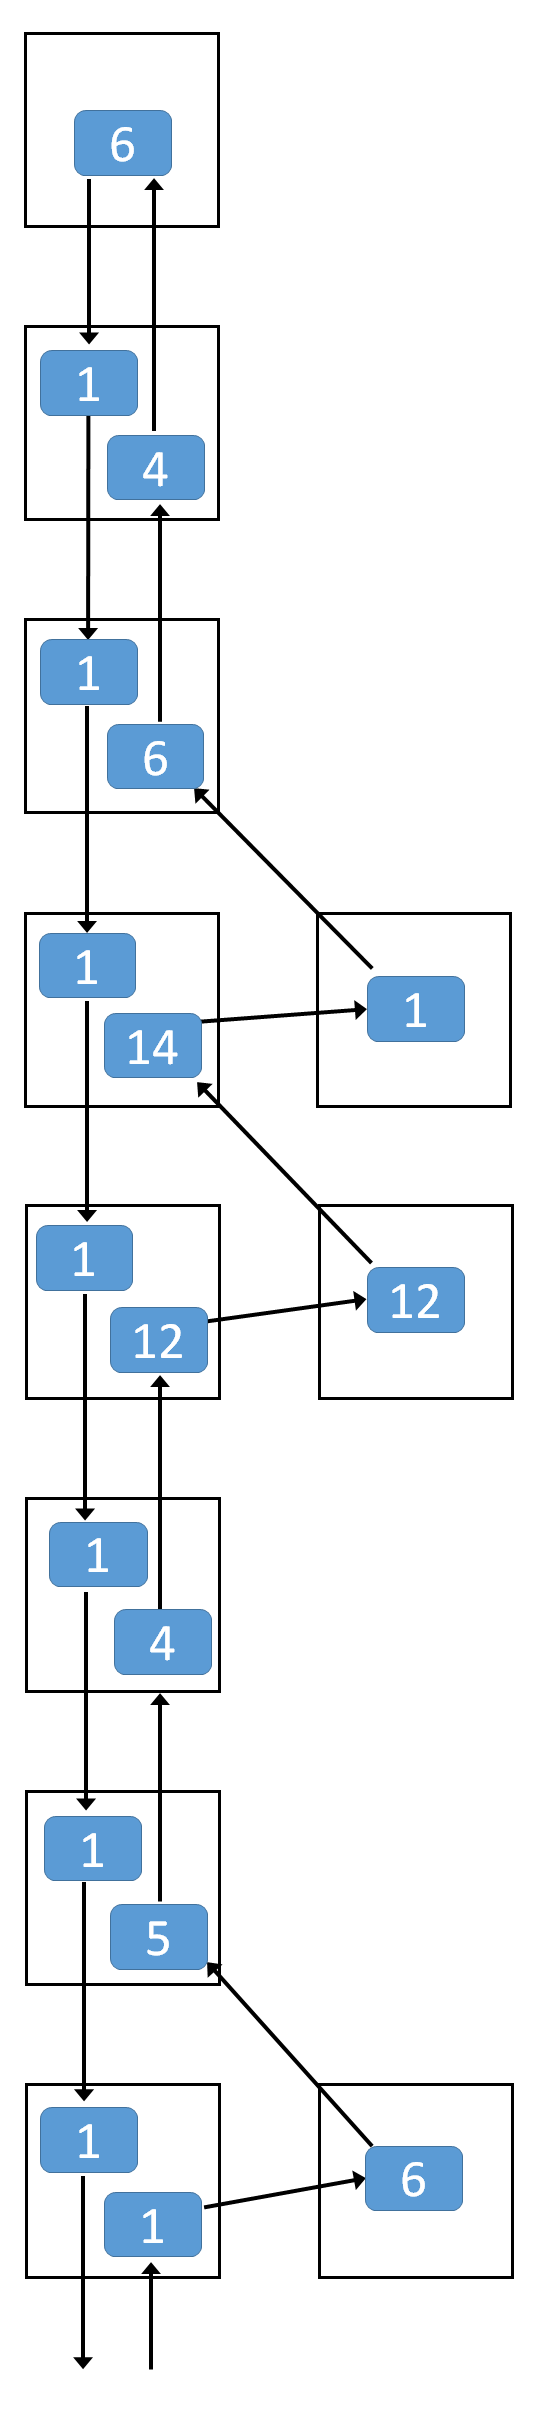
\includegraphics[scale=0.3]{./chap5/fig/1stage_data_path.eps}\\
          \hspace{2cm} (a)1ステージの場合
        \end{center}
      \end{minipage}

      % 2
      \begin{minipage}{0.5\hsize}
        \begin{center}
          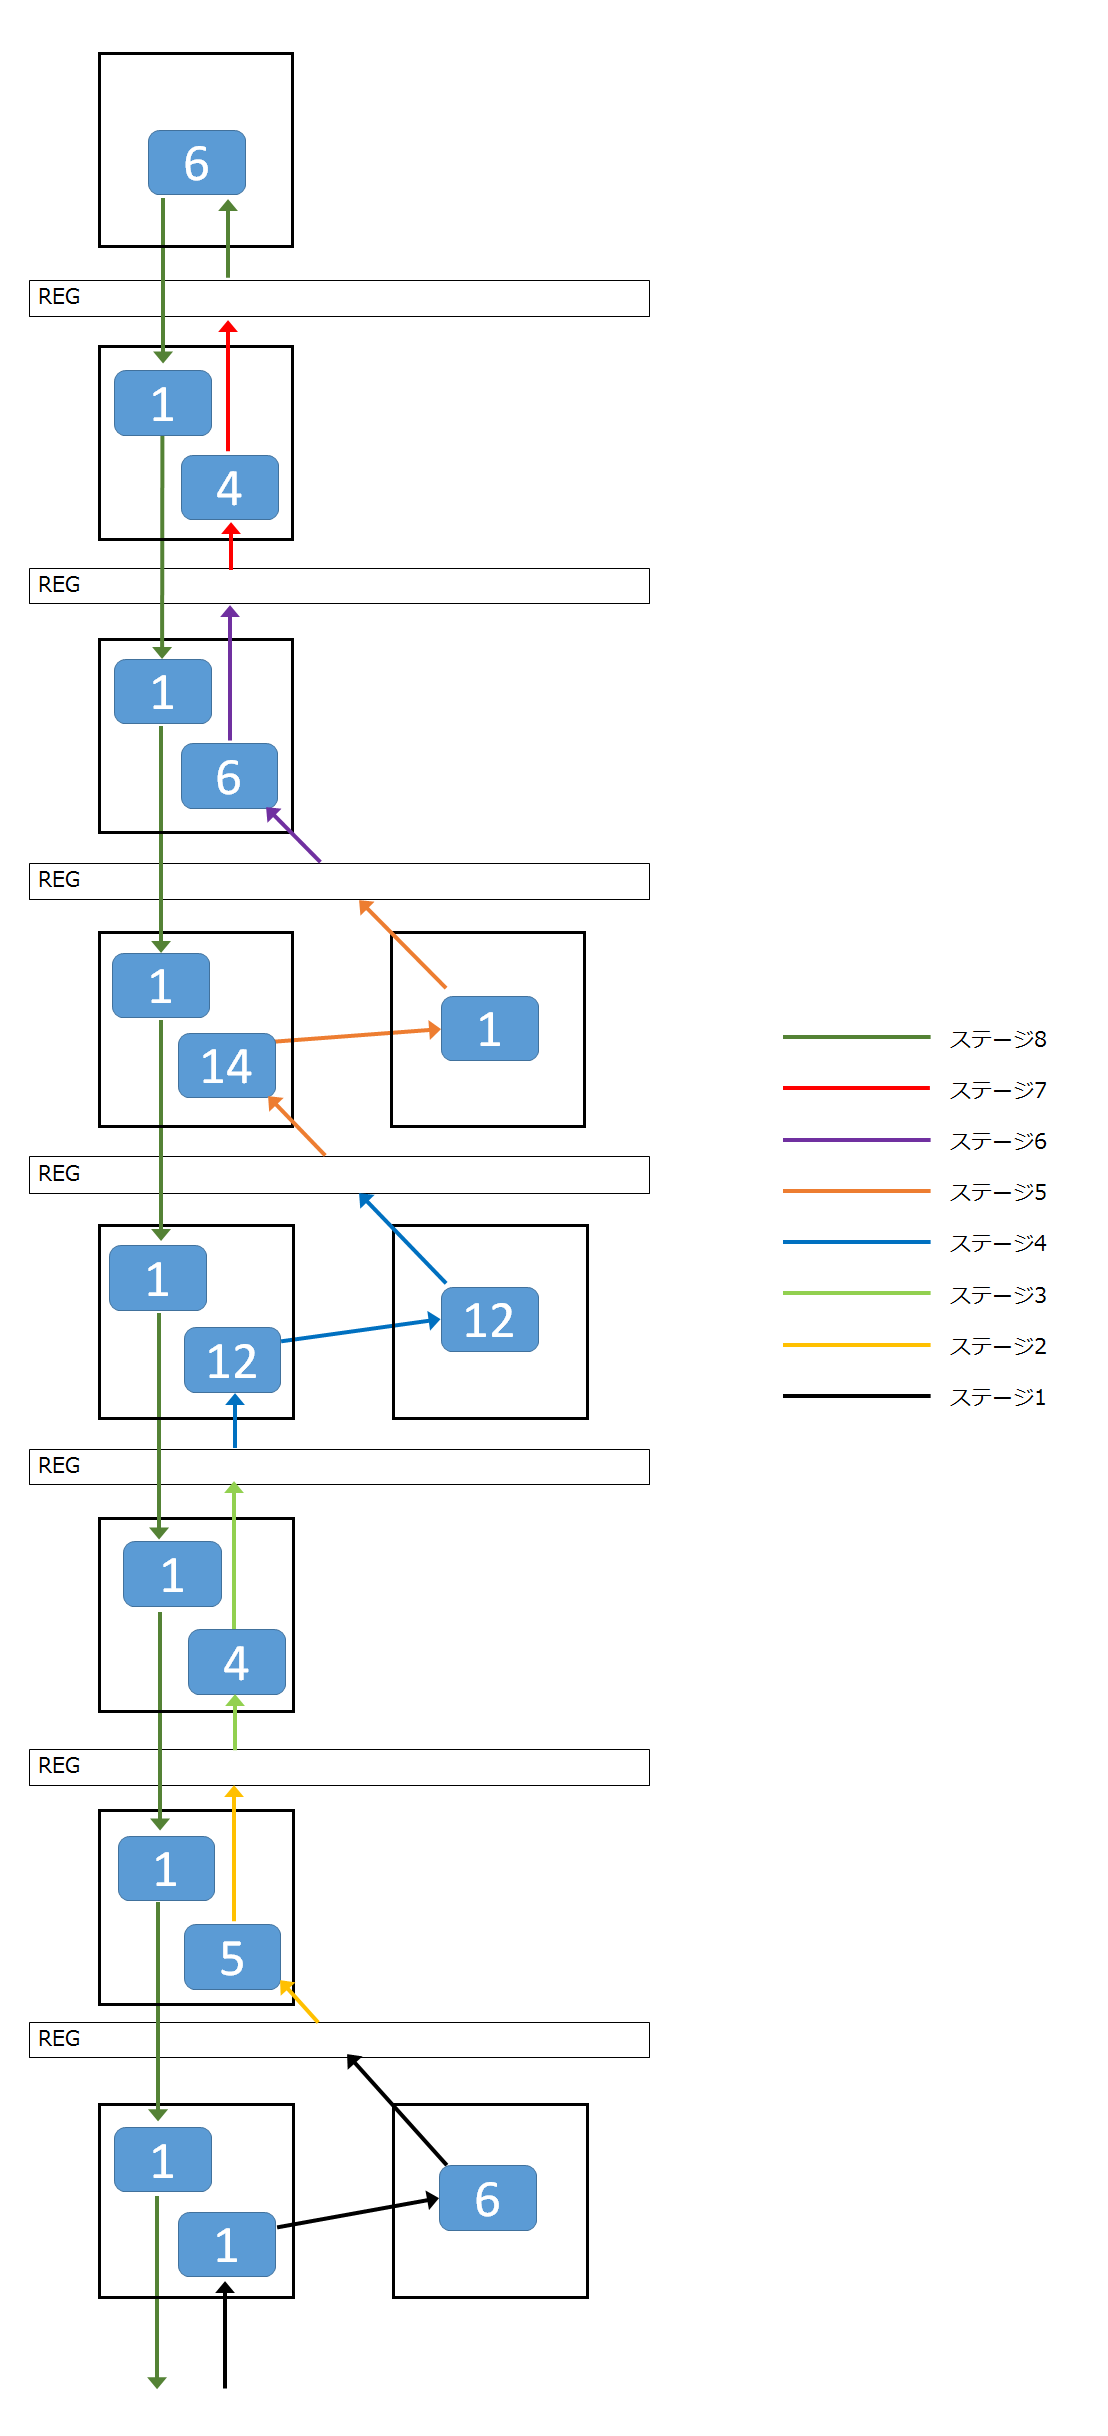
\includegraphics[scale=0.3]{./chap5/fig/8stage_data_path.eps}\\
          \hspace{2cm} (b)8ステージの場合
        \end{center}
      \end{minipage}


    \end{tabular}
    \caption{データパスと遅延の例}
    \label{fig:data_path_delay}
  \end{center}
\end{figure}

パイプライン分割しない場合の遅延時間を$D_1$とし、8段パイプラインの$n$番目のステージでの遅延を$D_8(n)$とする。これらは以下のように計算される。

\begin{eqnarray}
D_1 & = & 1 + 6 + 5 + 4 + 12 + 12 + 14 + 1 + 6 + 4 + 6 + 1 + 1 + 1 + 1 + 1 + 1 + 1 \nonumber \\
	& = & 78 \\
\nonumber \\ 
D_8(1) & = & 1 + 6 = 7 \\
D_8(2) & = &  5\\
D_8(3) & = & 4 \\
D_8(4) & = &  12 + 12 = 24 \\
D_8(5) & = &  14 + 1 = 15 \\
D_8(6) & = &  6 \\
D_8(7) & = &   4 \\
D_8(8) & = &  6 + 1 + 1 + 1 + 1 + 1 + 1 + 1 = 13
\end{eqnarray}

つまり、パイプライン分割しない1ステージの場合遅延が78であり、8ステージの場合最大遅延が24であると計算できる。


}